\section{Brief Data Visualisation}

A brief data visualisation helps reveal patterns, relationships, and potential anomalies that may not be apparent from raw numbers alone. By examining the plots, we can roughly estimate the result we expect to see, making a brief visualisation a good starting point in this assignment. A plot of the both datasets (\#13-13--13-1 and \#13-26--13-1 respectively) is shown in Figure \ref{fig:datasets} below. Each point represents a data sample, plotted using the two input features on the x and y axes, coloured according to its class label ($\pm$1)
\begin{figure}[H]
    \centering
    \begin{subfigure}[b]{0.47\textwidth}
        \centering
        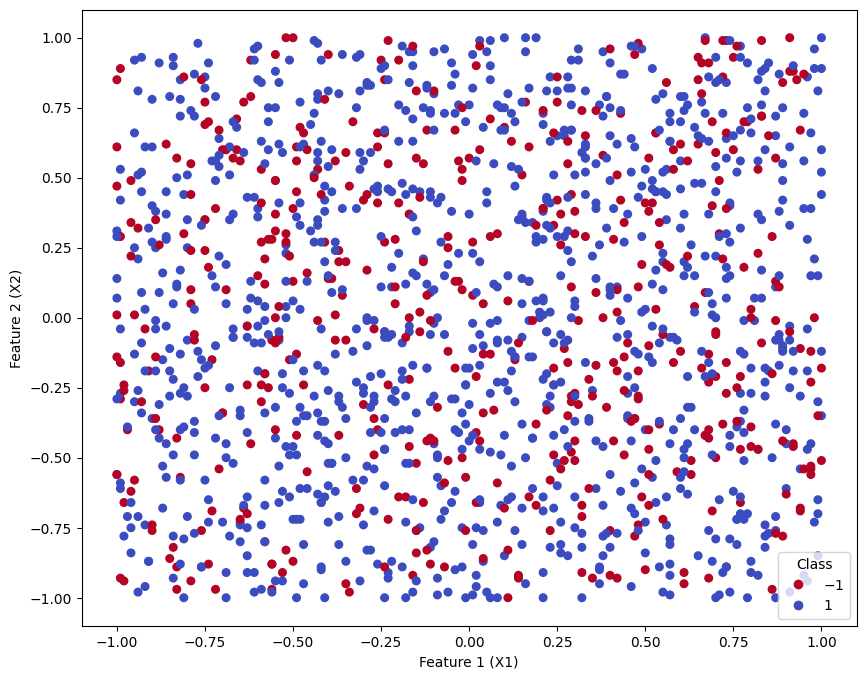
\includegraphics[width=\linewidth]{figures/dataset_1}
        \caption{Dataset 1}
        \label{fig:dataset1}
    \end{subfigure}
    \hfill
    \begin{subfigure}[b]{0.47\textwidth}
        \centering
        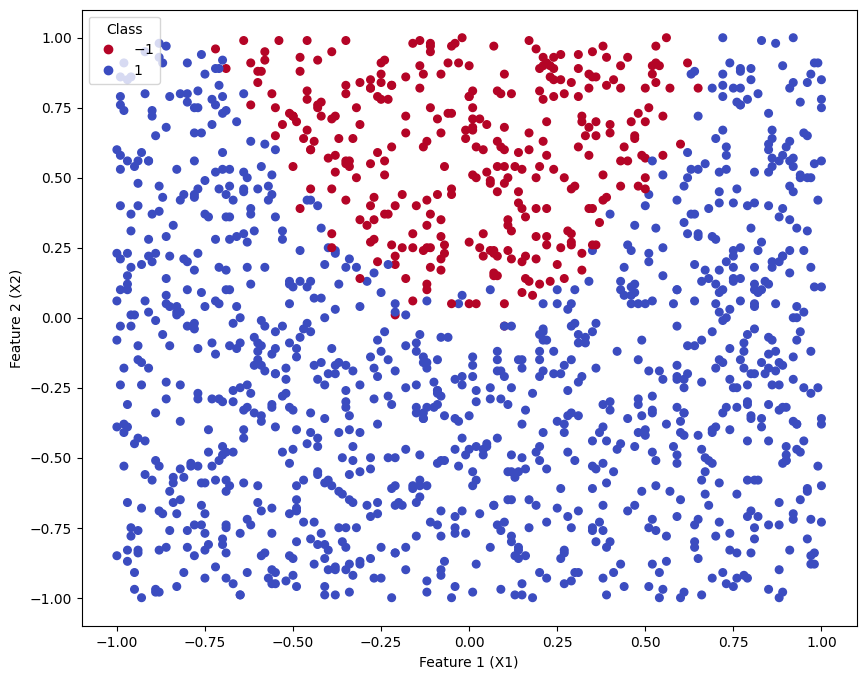
\includegraphics[width=\linewidth]{figures/dataset_2}
        \caption{Dataset 2}
        \label{fig:dataset2}
    \end{subfigure}
    \caption{Visualisation of Datasets}
    \label{fig:datasets}
\end{figure}
Figure \ref{fig:dataset1} shows overly noisy data with no clear separation between classes, and no clear relationship between features. From this, we can expect poor classification performance, as models are likely to struggle to find any meaningful decision boundary. 

The second dataset shown in Figure \ref{fig:dataset2} shows a clear separation between the two classes, with minimal overlap. Thus we can expect models to achieve much higher performance with this dataset. 